\documentclass[conference]{IEEEtran}

% --- IDIOMA ---
\usepackage[spanish, es-tabla]{babel}

% --- FUENTES (XeLaTeX) ---
\usepackage{fontspec}
\setmainfont{Liberation Serif}
\setmonofont{JetBrainsMono Nerd Font}

% --- CITAS IEEE ---
\usepackage[backend=biber,style=ieee,sorting=none]{biblatex}
\addbibresource{referencias.bib}

% --- UTILIDADES ---
\usepackage{graphicx}
\usepackage{float}
\usepackage{amsmath}
\usepackage{booktabs}
\usepackage[colorlinks=true,linkcolor=black,citecolor=black,urlcolor=blue]{hyperref}

% --- CÓDIGO ---
\usepackage{xcolor}
\definecolor{bg}{RGB}{40,44,52}

\usepackage{minted}

\setminted{
  style=monokai,
  bgcolor=bg,
  breaklines,
  breakanywhere=true,
  tabsize=2,
  fontsize=\footnotesize
}

\usepackage{csquotes}

\begin{document}



% --- INICIO DE LA PORTADA ---
\begin{titlepage}
    \centering
    \vspace*{0.5cm}
    
    % --- Escudo de la UV ---
    % Asegúrese de tener el archivo "escudo_uv.png" (o .jpg) en su carpeta del proyecto
    
\includegraphics[width=0.3\textwidth]{UV.png} \\ 
    \vspace{0.8cm}
    
    {\huge \textbf{Universidad Veracruzana}} \\
    \vspace{0.4cm}
    {\Large Facultad de Instrumentación Electrónica} \\ % Corregido: Instrumentación
    \vspace{0.2cm}
    {\large Ingeniería Biomédica} \\
    
    \vfill
    
    % Título de la Experiencia Educativa y Actividad
    {\Large \textbf{EE: Interfaces Hombre-Máquina}} \\
    \vspace{0.8cm}
    {\Large \textbf{Actividad 02: Botón de toque como dispositivo para una interfaz Hombre-Máquina}} \\
    
    \vspace{1.5cm}
 
    % Información de los Integrantes
    \begin{flushright} % Alineado a la derecha para un toque más profesional
        \textbf{Profesor:} \\
        Varela Lara Luis Julian \\
        \vspace{0.5cm}
        \textbf{Integrantes del equipo ``\textit{ES3.14}}'': \\
        Alfonso Gamboa Rubén \\
        Flores Montero Edsel Yetlanezi \\
    \end{flushright}
    
    \vfill
    
    {\large \textbf{Fecha:} \today} \\
    \vspace{1cm}
    {\small Xalapa, Enríquez, Ver.} % O la sede correspondiente
\end{titlepage}
% --- FIN DE LA PORTADA ---



% --- EL CUERPO DEL TEXTO (Automáticamente en dos columnas) ---

\section{Introducción al tema}
Durante el desarrollo de esta práctica se pondrá en práctica lo aprendido en clase anteriormente: el uso de la función \textit{milis} en lugar del uso de la función \textit{delay}, pues la función \textit{delay} detiene el programa una cantiad específica de milisegundos, con la desventaja que detiene todas las acciones durante su uso \cite{industrialshields_2020_millis}. Mientras que \textit{milis} no es una función de bloqueo \cite{industrialshields_2020_millis}; ésta devuleve los milisegundos que han pasado desde que se ejecutó el programa, pudiendo usar este valor para calcular la diferencia de tiempo que hay entre un evento y otro. Función a la que se le sacó ventaja para el desarrollo de esta actividad.

\section{Dearrollo de la actividad}
  \subsection{Desarrollo del código}
  Para desarrollar el código primeramente se descomprime ComandosRS232.zip (descargado de la Actividad 01), obteniendo así nuestra primera dificultad: el fichero ComandosRS232.exe.

  Para poder ejecutar ComandosRS232.exe se instala wine-11.4 (Staging). Fallando e inutilizando la GUI (figura \ref{fig:ComandosRS232}), por lo que se opta por trabajar con arduino tui.

  Durante el desarrollo del código no se contaba con el material, sin embargo se sabía de atemano que su comportamiento no debía ser muy diferente de lo de un botón pulsador \cite{keim_2016_capacitive}, por lo que para las pruebas, se iban a realizar con botones pulsador.

  Primeramente en el código se declaran funciones y variables que se van a ocupar posteriormente: BotonUp y BotonDown van a ser asignados a los pines 2 y 3 respectivamente, 

  Se crean variables con el prefijo \textit{``unsidgned long'' }, estas variables nos van a servir para guardar \textit{tiempo}, por lo que se usa \textit{long} para indicar que es un número muy grande, y como no vamos a trabajar con números negativos, se indica el prefijo \textit{unsigned} (sin signo), pudiendo guardar números más grandes pero sin signo.
  
  Se crea una función llamada \textit{calcularIntervalo()}, que retornará un número entero (\textit{int}) y que recibe de parametro tiempo (con las mismas condiciones que hemos usado para las variables del principio), esta función la queremos para decirle al Arduino la velocidad (en milisegundos) a la que queremos que incremente la variable \textbf{valor}.

  Dentro del setup, le decimos a arduino que queremos ocupar 9600 baudios (estándar en arduino) y que queremos que los pines 2 y 3 serán inputs.

  Dentro del loop leemos si los botones están presionados, guardamos esta información en variables booleanas, pues nos permiten usarlas como condicionales, facilitando la lectura del código. Además en esta parte añadimos una variable de control llamada  \textit{ahora}, que nos va a permitir saber \textit{en que momento de milisegundo nos encontramos ahora mismo desde que se inició el programa.}

  \textbf{Primer condicional: Si ambos botones son presionados.} Este primer condicional nos permite conocer si ambos botones se encuentran presionados, si esta oración es cierta, cambiamos el estado de amobos a \textit{no presionados}, probocando que el programa no haga nada.

  \textbf{Segundo condicional: si UP es presionados.} 
  \begin{enumerate}
    \item Se anida un \textit{if} que nos permite registrar en la variable de control \textit{upPresionado} a \textit{verdadero} si esta no lo estaba, guardando en el proceso, cuando fue presionado y el utlimo cambio.
    \item Se calcula cuanto tiempo lleva presionado el botón: restando el tiempo de ahora, menos el momento en el que se presionó.
    \item Con la función anterior de \textit{calcularIntervalo()} se le asgina un intervalo de tiempo en el que tiene que imprimir el valor.
    \item Finalmente, si la diferencia de los cambio, supera al intervalo (dado por el tiempo presionado), se imprime el valor. y se regisra el último cambio. Este último \textit{if} es el causante del aumento de la velocidad, al evaluar constantemente \textit{¿Debo imprimir ahora mismo?}
  \end{enumerate}
  
  Finalmente para el \textbf{Tercer condicional} principal se repite la misma lógica que en el segundo, pero aplicado para el boton para bajar el valor.

  \begin{figure}[t]
    \centering
    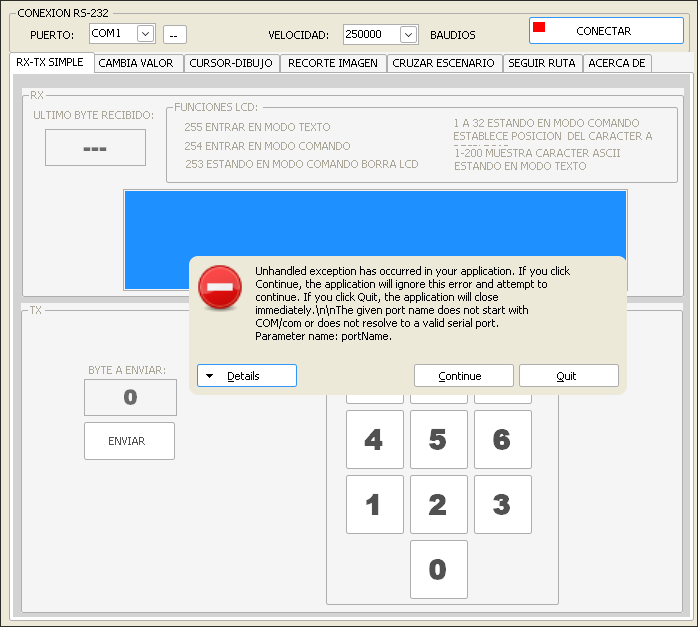
\includegraphics[width=\linewidth]{2026-03-13_21:55:54.png} % \linewidth se ajusta a la columna
    \caption{Falla del programa ComandosRS232}
    \label{fig:ComandosRS232}
  \end{figure}


  \subsection{Armado del circuito}
  Para el armado del circuto Se ocupó de un Arduino Uno, una protoboard, jumpers, los botones capacitivos fueron conectados respetando sus etiquetas VCC, GND y I/O:
  \begin{enumerate}
    \item Los pines de VCC fueron conectados en común al puerto de 5v del Arduino Uno.
    \item Los pins GND fueron conectados en común al puerto GND del Arduino Uno.
    \item El pin I/O del primer botón se conectó al puerto digital 2 del Arduino, este botón será para incrementar el valor.
    \item El pin I/O del segundo botón se conectó al puerto digital 3 del Arduino, este botón será para decrementar el valor.
  \end{enumerate}

  \begin{figure}[t]
      \centering
      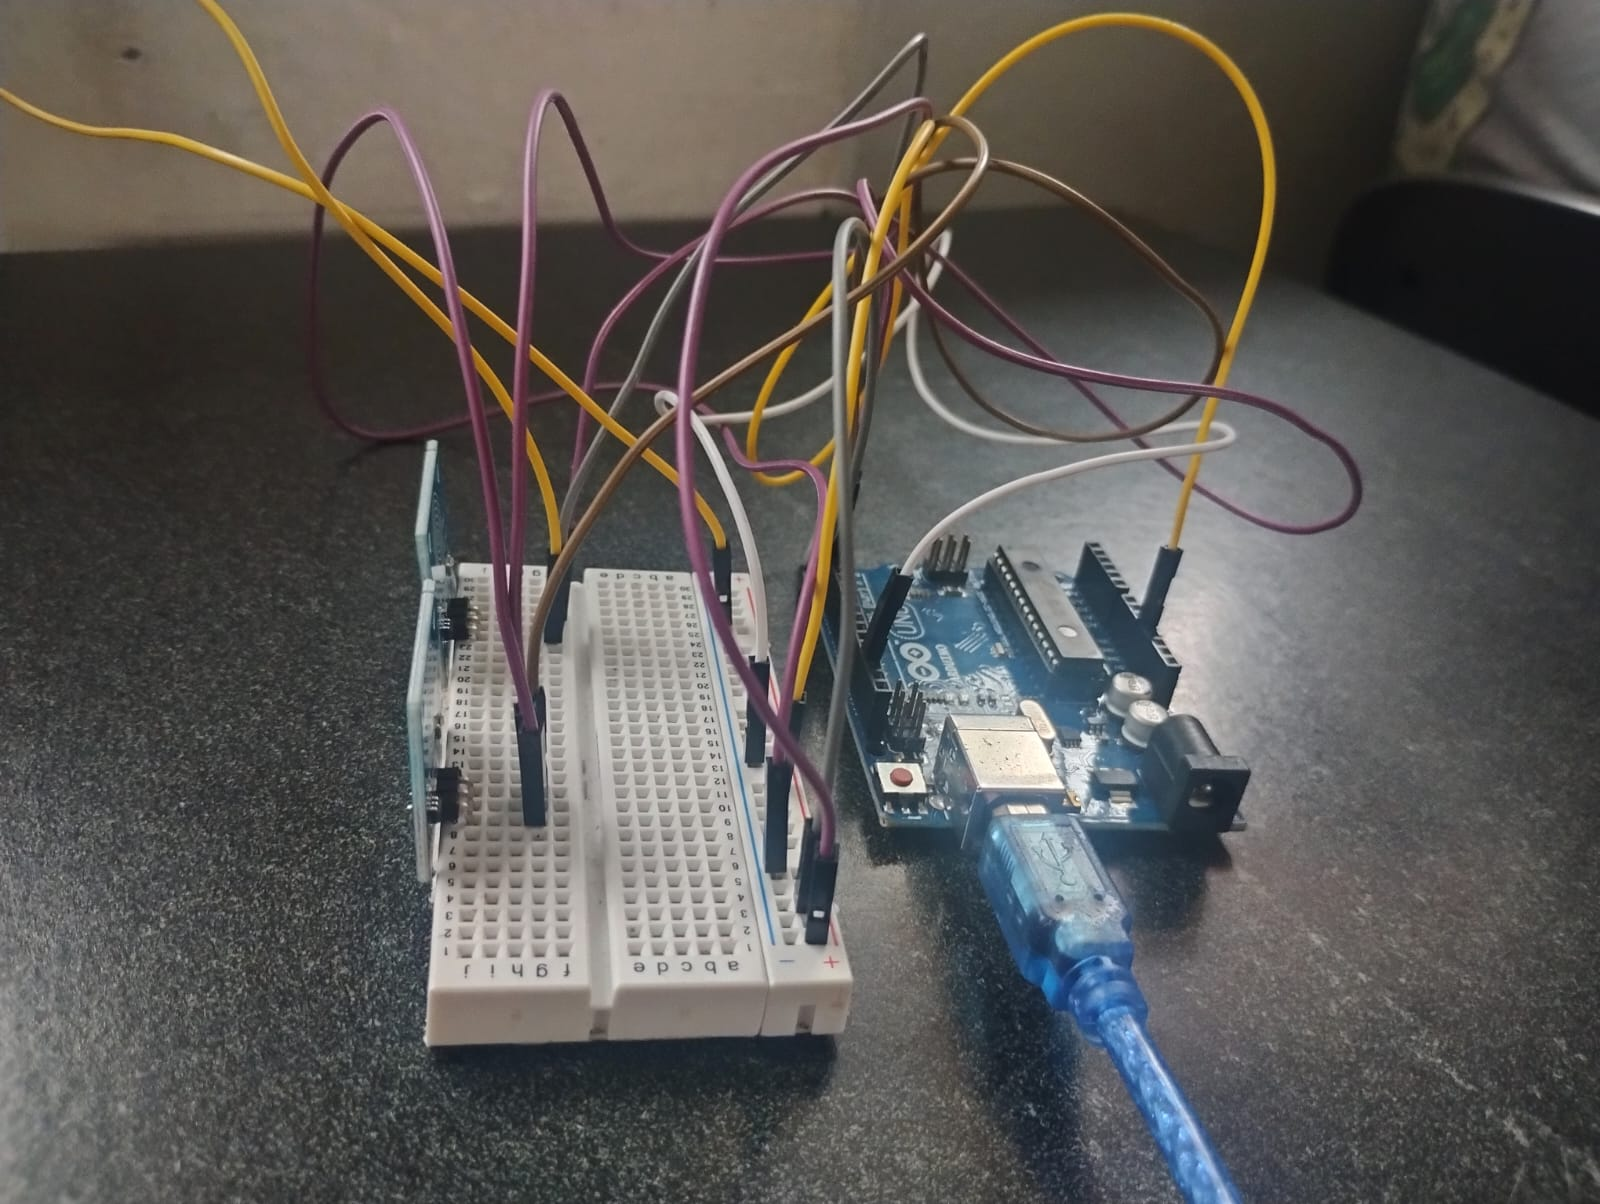
\includegraphics[width=\linewidth]{circuito.jpg} % \linewidth se ajusta a la columna
      \caption{circuito armado}
      \label{fig:circuito}
    \end{figure}

  \newpage
  \subsection{Código completo}
    A continuación se deja el código completo usado durante el desarrollo de esta actividad:
    \inputminted{cpp}{Act02.ino}



\section{Conclusiones}
La mayor dificultad para el desarrollo de esta práctica fue el mal funcionamiento del \textbf{ComandosRS232.exe} dentro del entorno linux, lo que llevó a una malinterpretación de funciones y objetivos por parte del equipo, por lo que se optará por el uso de maquinas virtuales para el desarrollo de las futuras actividades.

El uso de la función \textit{milis}, permite un uso continuo del microcontrolador Arduino Uno sin necesidad de hacer pausas que congelen al microcontrolador. Permitiendo un uso continuo de éste para otras tareas.
El uso de botones touch son una alternativa moderna e ingeniosa a los botones que se pulsan, evitándonos los problemas comunes del polvo y el desgaste del resorte.

\newpage{}
\section{firma de revisión}
\begin{figure}[h]
    \centering
    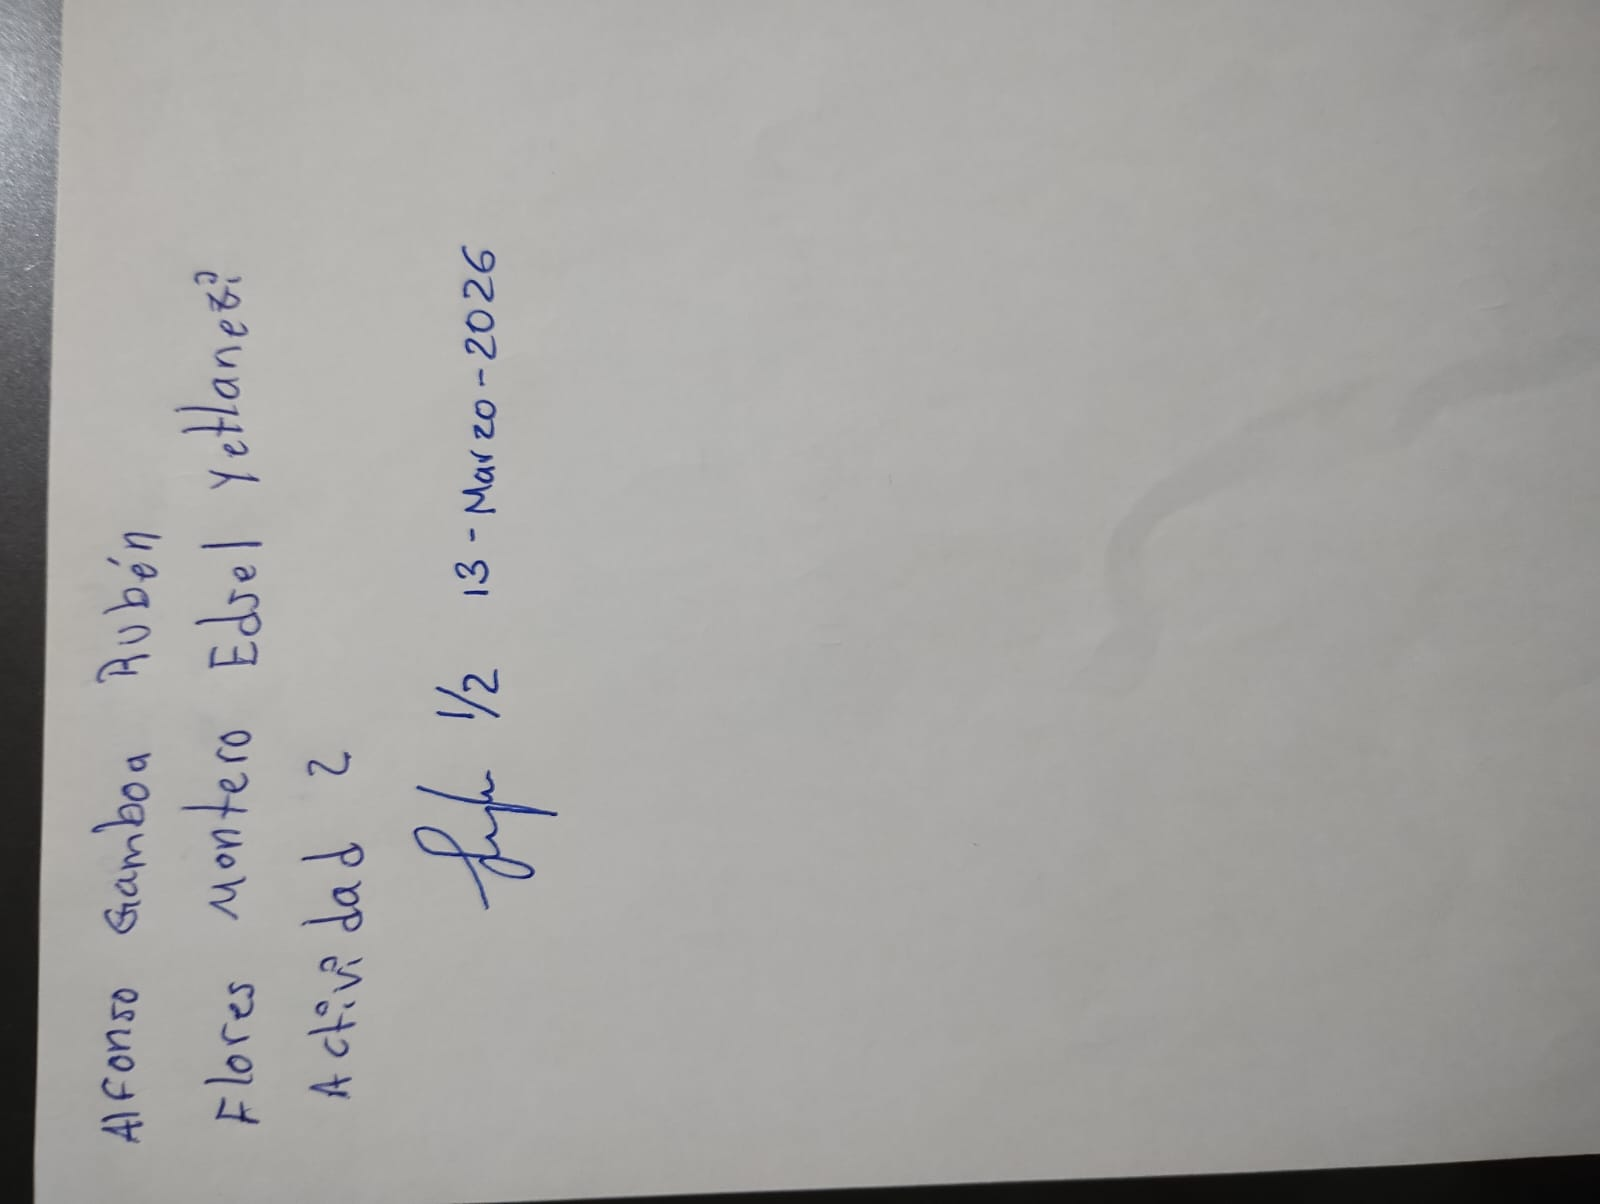
\includegraphics[width=\linewidth, angle=-90]{Firma.jpg} % \linewidth se ajusta a la columna
    \caption{Firma de revisión}
    \label{fig:Firma}
\end{figure}



% --- REFERENCIAS ---
\printbibliography

\end{document}
